\documentclass[a4paper]{article}

\usepackage[fancy]{template}
\usepackage{survival-pack}

\setup{%
  subject={Datanet},%
  assignment={Assignment 1},%
  date={29 April, 2013}%
}
\setupLocation[short=DIKU]{Datalogisk institut, Københavns Universitet}
\setupAuthor[addendum={ \ }]{Rasmus Wreidt Larsen \\ Martin Bjerregaard \\ Jonas Brunsgaard}

\newcommand{\commandstyle}[0]{{\ttfamily\textbackslash}}
\newcommand{\command}[1]{\texttt{\textbackslash #1}}

\begin{document}

\maketitle
\thispagestyle{first}
\newpage

\section{Theoretical part}
\subsection{Store and Forward}
\subsubsection{Processing and delay}
In addition to propogation delay we have

\begin{description}
    \item[Processing delay] A delay caused by the routers in the network,
        due to the requirement of examining the packet's header information to
        determine where to direct the package.
    \item[Queue delay] If more packets are going into the same link, the
        router forms a queue, where a packet is hold until it is
        transmitted, this delay is called a queue delay.
    \item[Tranmission delay] The time required to push all of the packet's bits
        into the link. This is often the most most significant delay.
\end{description}

% Calculations for the subsection on transmission speed
\subsubsection{Transmission speed}
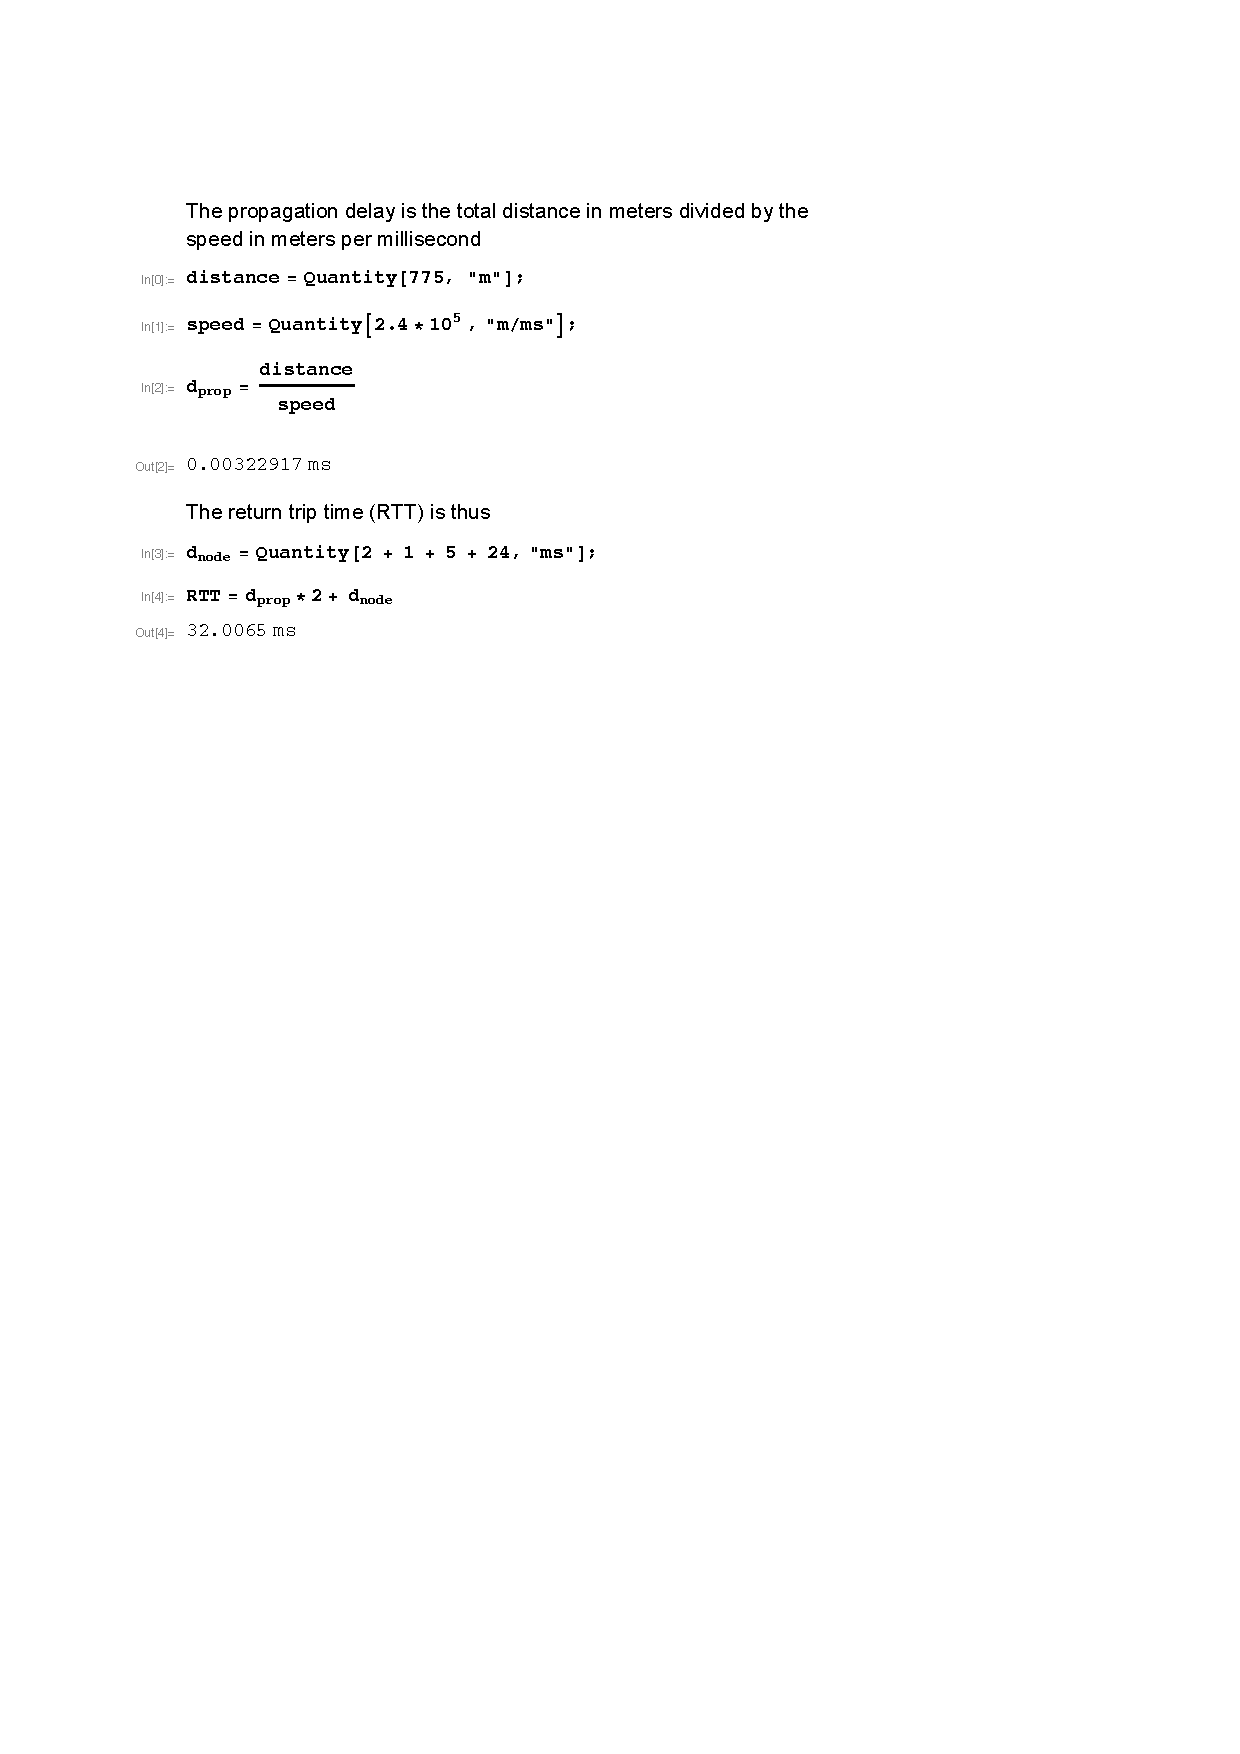
\includegraphics{../calc1.pdf}
\newpage
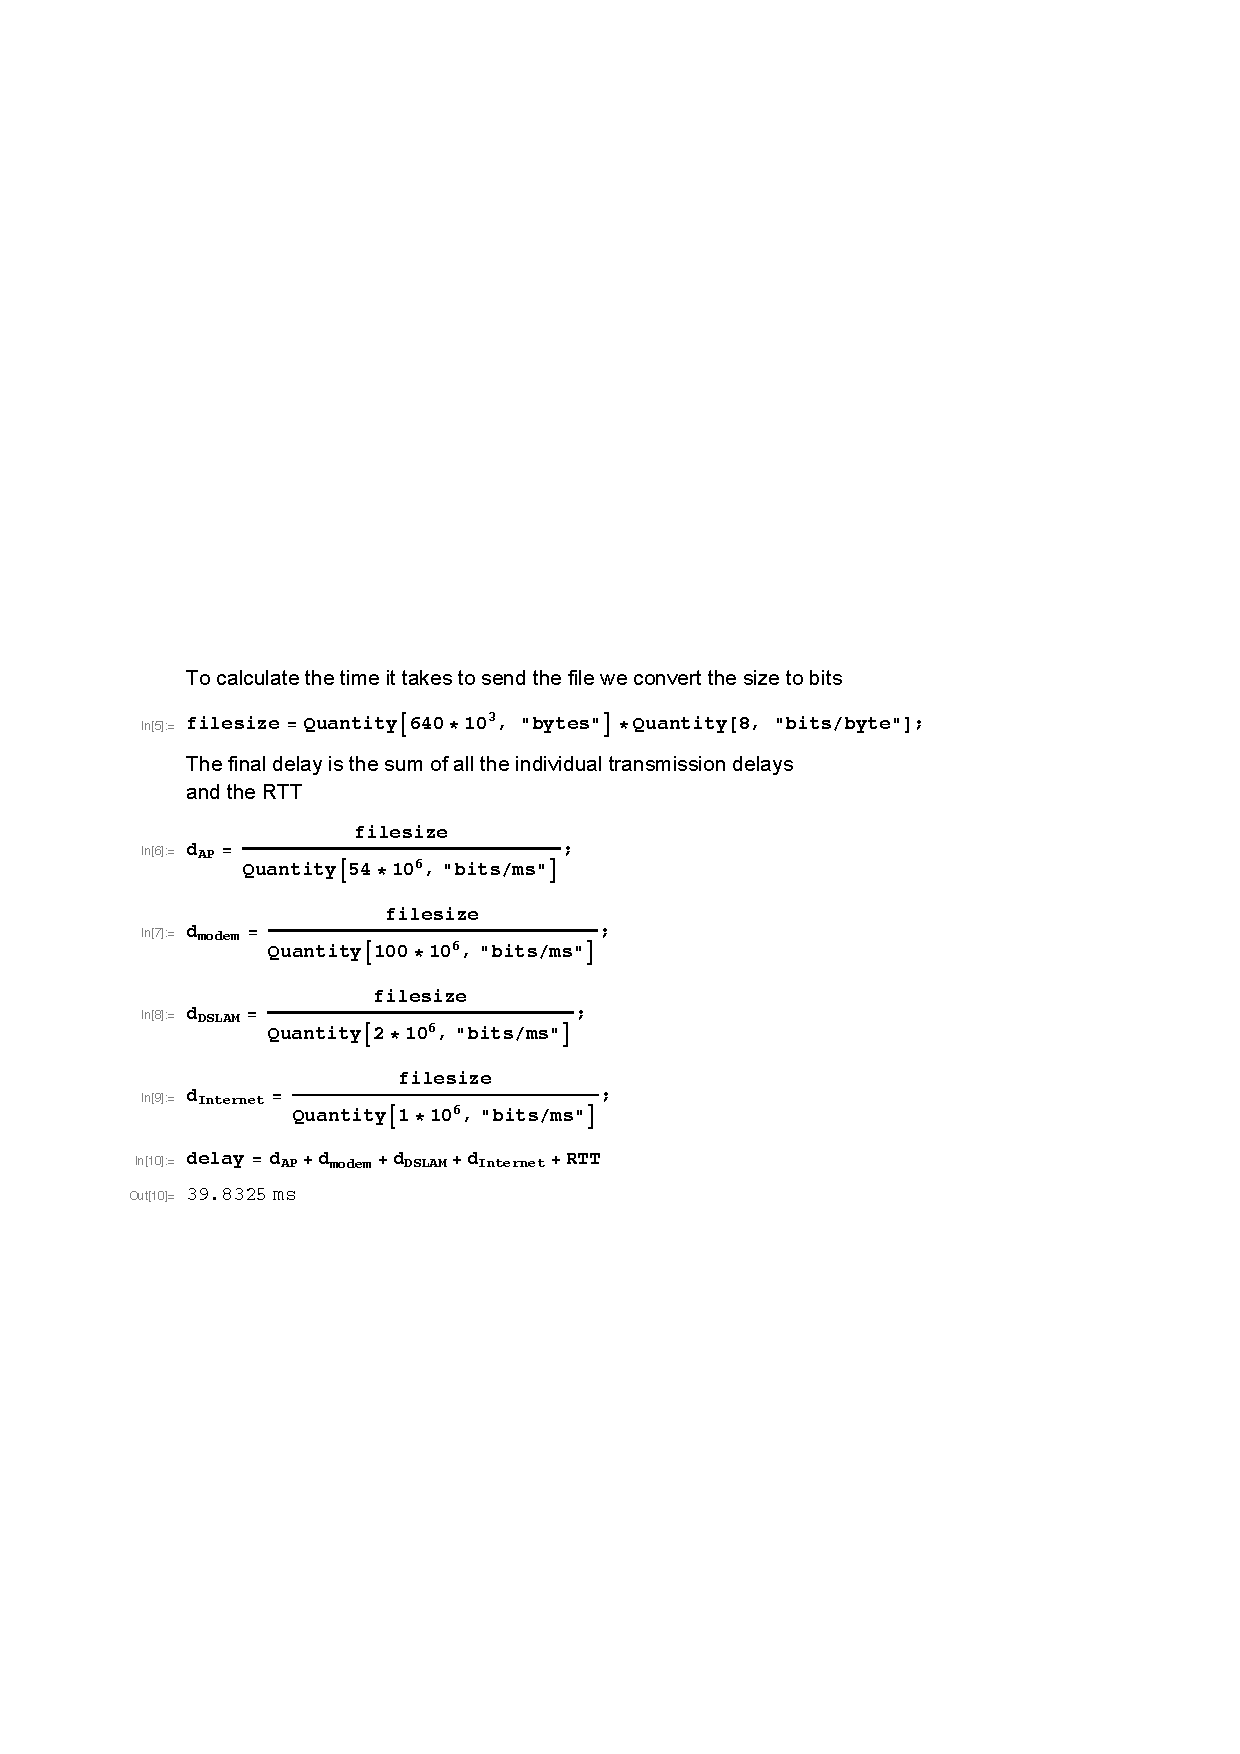
\includegraphics{../calc2.pdf}

\subsection{Buffers and latency}
\begin{description}
    \item[Part 1] The link behind the DSL modem is limited to 54 Mb/s by the
        wireless connection, but is significantly faster than the 2Mb/s upload
        speed of the modem. Given a continuous upload burst it will be filled
        in approx. 78.7 milliseconds, leading to further packets being dropped.
        This results in a maximum packet delay that is infinite. All packets
        from the student will then be discarded.
    \item[Part 2] The \emph{Bandwith-delay product} can be seen as a
        measurement of the ``volume'' of the network link, describing how much
        data that can be on the link at any point in time. TODO: Why good
        measure, and what are consequences?
\end{description}

\subsection{HTTP}
\subsubsection{HTTP semantics}
\begin{description}
    \item[Part 1] The request method field is required to indicate the desired
        action to be performed on the server. The GET method means to retrieve
        the information identified by the Request-URI, and the POST method
        requests that the server accepts the entity enclosed in the request as
        a new subordinate of the Request-URI. In practice both GET and POST can
        be used to post data to the server through query parameters, but only
        POST can contain a enclosed entity, Query parameters to requests are
        often visible in the http server's log files etc, therefore posting
        sensitive data using query parameters is very bad practice. Instead the
        enclosed entity in POST is used in practice to meet this problem.

    \item[Part 2] The following definition of the Host header is taken from
        section 14.23 of RFC 2616, and clarifies that the Host header is
        essential because it allows a server or gateway to differentiate
        between internally ambiguous URLs, and thereby enabling virtual
        hosting.

        The Host request-header field specifies the Internet host and port
        number of the resource being requested, as obtained from the original
        URI given by the user or referring resource (generally an HTTP URL, as
        described in section 3.2.2). The Host field value MUST represent the
        naming authority of the origin server or gateway given by the original
        URL. This allows the origin server or gateway to differentiate between
        internally ambiguous URLs, such as the root "/" URL of a server for
        multiple host names on a single IP address).

    \item[Part 3] When we enter \url{http://google.com} into a brower we are
        redirected to \url{http://www.google.dk}. Now we use \texttt{nc} to see
        what is happening behind the scenes.

\begin{lstlisting}
~ nc google.com 80
GET / HTTP/1.1
Host: google.com

HTTP/1.1 301 Moved Permanently
Location: http://www.google.com/
Content-Type: text/html; charset=UTF-8
Date: Fri, 03 May 2013 21:30:51 GMT
Expires: Sun, 02 Jun 2013 21:30:51 GMT
Cache-Control: public, max-age=2592000
Server: gws
Content-Length: 219
X-XSS-Protection: 1; mode=block
X-Frame-Options: SAMEORIGIN

<HTML><HEAD><meta http-equiv="content-type" content="text/html;charset=utf-8">
<TITLE>301 Moved</TITLE></HEAD><BODY>
<H1>301 Moved</H1>
The document has moved
<A HREF="http://www.google.com/">here</A>.
</BODY></HTML>
\end{lstlisting}
We get the response code 302 (Moved Permanently) and a Location header field in
the response. The browser therefore redirects to \url{http://www.google.com}.
But we end up at \url{http://www.google.dk}, so we may have been redirected
again. Again we use \texttt{nc} to check.

\begin{lstlisting}
~ nc www.google.com 80
GET / HTTP/1.1
Host: www.google.com

HTTP/1.1 302 Found
Location: http://www.google.dk/
Cache-Control: private
Content-Type: text/html; charset=UTF-8
Set-Cookie: PREF=ID=9afb5378969d7c0d:FF=0:TM=1367617467:LM=1367617467:S=3dVXq7FD_dcXVzbV; expires=Sun, 03-May-2015 21:44:27 GMT; path=/; domain=.google.com
Set-Cookie: NID=67=S95px1WKn7E0DH9nAavEDvvcQuLveGiNyNpua3hqKDSaFFvuhhTUu 534pV86HHQOnca8Yp9odT4KQp-Ijh-qUIVuXcZQuea6nso1cgyg47JOo3_JvYvLbKXPePsa9E6q; expires=Sat, 02-Nov-2013 21:44:27 GMT; path=/; domain=.google.com; HttpOnly
P3P: CP="This is not a P3P policy! See http://www.google.com/support/accounts/bin/answer.py?hl=en&answer=151657 for more info."
Date: Fri, 03 May 2013 21:44:27 GMT
Server: gws
Content-Length: 218
X-XSS-Protection: 1; mode=block
X-Frame-Options: SAMEORIGIN

<HTML><HEAD><meta http-equiv="content-type" content="text/html;charset=utf-8">
<TITLE>302 Moved</TITLE></HEAD><BODY>
<H1>302 Moved</H1>
The document has moved
<A HREF="http://www.google.dk/">here</A>.
</BODY></HTML>
\end{lstlisting}
This time we get a 302 (Found) response code, and the location header field
matchs the destination of our browser. Seems like the browser redirected us a
second time. Now it all makes sense.

The response codes are obviously important to categories and  structure
feedback from the server. This formalisation, allows browsers and other
software to make automated decisions (eg redirecting in case of 3xx or exclude
indexing in case of 4xx) based on the respons.
\end{description}

\subsubsection{HTTP headers and fingerprinting}
\begin{description}
\item[Part 1] It is a way of saving information on the client side and sending
    it back to the server in future requests. The Set-Cookie header field will
    imply that the browser creates a cookie (if cookies are enabled). The
    client can now ask for a new resource on the same host and the cookie will
    be send with the new request.

    A session token is a unique identifier used to identify a session, the
    client usually stores and sends the token as an HTTP cookie, in such cases
    the cookie is used as an unique identifier.

\item[Part 2] Headers that might leak sensitive information can include the Server and X-Powered-By (used by PHP and others). These
    headers gives the client information on the server infrastructure that is being used to host the page. The headers may be disabled
    in the configuration files for most servers.
\item[Part 3] Because the ETag may contain arbitrary values, it can hold a unique identifier given to a user. This identifier
    is then sendt to the server whenever the page is requested. Instead of checking whether the page has been modified, the server
    will then return the whole page and the same ETag identifier. This ensures that the identity value is persisted in the brower's
    cache, and enables tracking of users.

    If one also wishes to enable caching of pages, a specific resource (an image) can be injected into every page. This resource could handle
    the tracking using ETags, and the rest of the pages could use ETags for simple caching.
    %\url{http://www.arctic.org/~dean/tracking-without-cookies.html}
\end{description}

\subsubsection{The case of Deep Packet Inspection}

\begin{description}
    \item[Part 1] ``3'' could have filtered all requests to
        \texttt{grooveshark.com} by dropping all packets with a destination
        host being an IP belonging to that domain. This could be done in the
        network layer without breaking the layering model of the network stack.
    \item[Part 2] This is a violation of layering in networks because a layer
        is inspecting and modifying the data passing in a layer above it. To
        stop this and enforce the layering we may encrypt the HTTP stream by
        using HTTPS (SSL).
\end{description}


\section{Practical part}
\subsection{Socket Programming}

\subsubsection{Question 1}

Restricting the messages size to \texttt{BUFFER\_SIZE}, simplifies receiving data, as one only need to have a buffer of the specified size. But it also puts a strict limit on the amount of data that can be sent.
If one should take the token based approach, a good candidate for the token could be the \texttt{EOT} character, (ASCII number 4), meaning ``end of transmission''.
Using a specific buffer size is required by the socket API, so one would need to use a combination of the two. If the last character recieved is not the token for end of message, one simply recieve data once more. Each part of the message then needs to be concatenated in the end to look at the whole message.
For this particular case, limiting message size to 1024 should not be a big problem, as message sizes should be fairly small -- with the exception that one can make arbitrability large ECHO commands.

\subsubsection{Question 2}

As the protocol is stateless, as described below, we can just close the socket on the server. In our implementation the client program is terminated if the socket dies, so the client has to reconnect anyway.

\subsubsection{Question 3}

Each command in the protocol was manually tested to verify expected behavior. Both client and server handles malformed requests,
by only reacting on the specified commands. To increase robustness, clients can handle situations where the server is not up
or crashes within a session. The client does not handle malformed responses, it just prints whatever it gets.

To increase the robustness of the server one might adopt a threaded architecture, where every connecting client gets their own thread.
This could also enable several users to connect to the server in parallel. A crash in one thread would then kill the thread, but not
interfere with the working of the other threads.

The client could be crashed by sending responses containing control bytes back to the client. One might filter all the bytes that
the client receives and only display those that are in a whitelist. However this change changes the output on the client side, and
is arguably a violation of the lack of restrictions on messages that the protocol handles.

TODO: other basic steps?

\subsubsection{Question 4}

The protocol is stateless, because the server does not need to maintain any information about the client. In our implementation we keep the socket open, but the protocol does not require us to do so.


\end{document}
